\section{Analysis / Our approach} % (fold)
\label{sec:own_approach}

The \crowdre{} dataset is available in form of a MySQL database dump, but the tables can also be downloaded separated into several \textit{.csv} files\footnote{\url{https://crowdre.github.io/murukannaiah-smarthome-requirements-dataset/}, last visited 2020-01-15}. For our research, we were only interested in the pure requirement sentences (without any ratings, or user characterization added to the data). We could therefore reconstructed the sentences from the \textit{requirements.csv} file only, which is included in the downloaded data.

To have a benchmark for the approaches we want to use we need a labelling at the dataset that we can use to rate how good the topic modelling worked. At first we checked if we can use the tags as soft labelling for the requirements but unfortunately most of them are only matched once (Total tags: 2116, tags that only occur once: 1562). We also checked the amount of requirements represented by the most common tags. 

\begin{figure}[h]
  \centering
    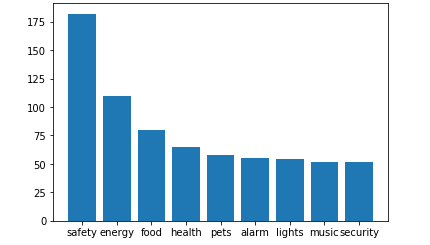
\includegraphics[width=0.8\textwidth]{screenshots/tag_analysis.png}
    \caption{Tag occurence and coverage of the requirements}
    \label{fig:tag_analysis}
\end{figure}

In \autoref{fig:tag_analysis} it is obvious that the high amount of tags that only occur once lead to the fact that the relation between requirements is not working good. The variety of tags that may be assigned to the same topic is very high and the low coverage of requirements with the top 9 tags makes the tags not suitable for the soft labelling. So we checked the domains that were assigned to the requirements. The domains are separated into five groups: Health, Energy, Entertainment, Safety and Other. For the \grqq{}Other\grqq{} there are again user defined specific domains, but we focus on the five top level domains for our labelling.

\subsection{NLP Preprocessing Pipeline} % (fold)
\label{sub:own_pipeline}

\begin{figure}[ht]
  \centering
    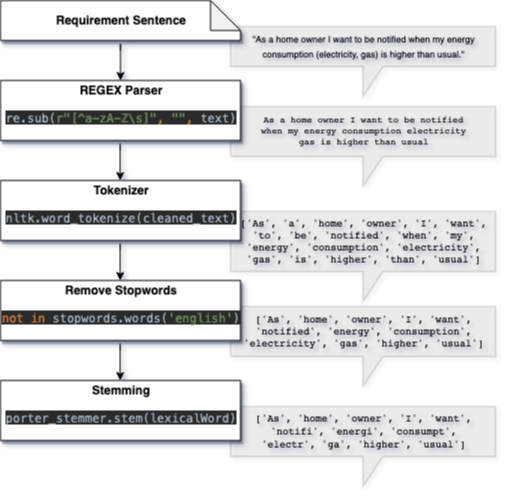
\includegraphics[width=\textwidth]{figures/NLP Pipeline.png}
    \caption{Our NLP Preprocessing Pipeline and an exemplaric requirement sentence.}
    \label{fig:nlp_pipeline}
\end{figure}

As initially described in \autoref{sec:nlp} we preprocessed our requirement documents using an NLP pipeline as shown in \autoref{fig:nlp_pipeline}. Implementing our solution in Python and following the common practice as suggested in \cite{ferrari_natural_2018}, we made use of the NLTK library\footnote{\url{https://www.nltk.org/}, last visited 2020-01-18} to perform the NLP techniques we needed for our analysis. As some of the requirements sentences contained special characters, some initial data cleansing was necessary, to remove these special characters (i.e. spaces, dots, apostrophes, slashes) as they would have otherwise been ranked in the later used bag of words. We used regular expressions as provided by the Python standard library in order to do so. For the tokenization, the stop-word-removal and the stemming we used the functions provided by the NLTK API.
% subsection preprocessing (end)

\subsection{LDA Approach} % (fold)
\label{sub:own_lda}
After we developed our pre-processing pipeline for the dataset and some basic analysis on the data we have we decided to use the LDA for a first topic modelling. The idea was to have another approach in the first step that we can use as intermediate result for the data and also to compare it to the result of the neural network to have some kind of benchmark or basis for a performance comparison.


For our LDA approach we used our preprocessed requirements. To apply an LDA to the data we need an array of arrays where each inner array represents a single requirement (so in this dimension it has 2966 entries). each word in the requirements needs to be replaces by a number that can be processed by the LDA. So we first applied a bag-of-words which calculates a relative weight for the single words. the next step is rating the words with the TF-IDF. After these steps we have a prepared matrix that contains the data that now can be processed by the LDA.

\begin{figure}[bht]
    \subfigure[LDA Plot with colors to topics\label{fig:lda-tf-idf-topics}]{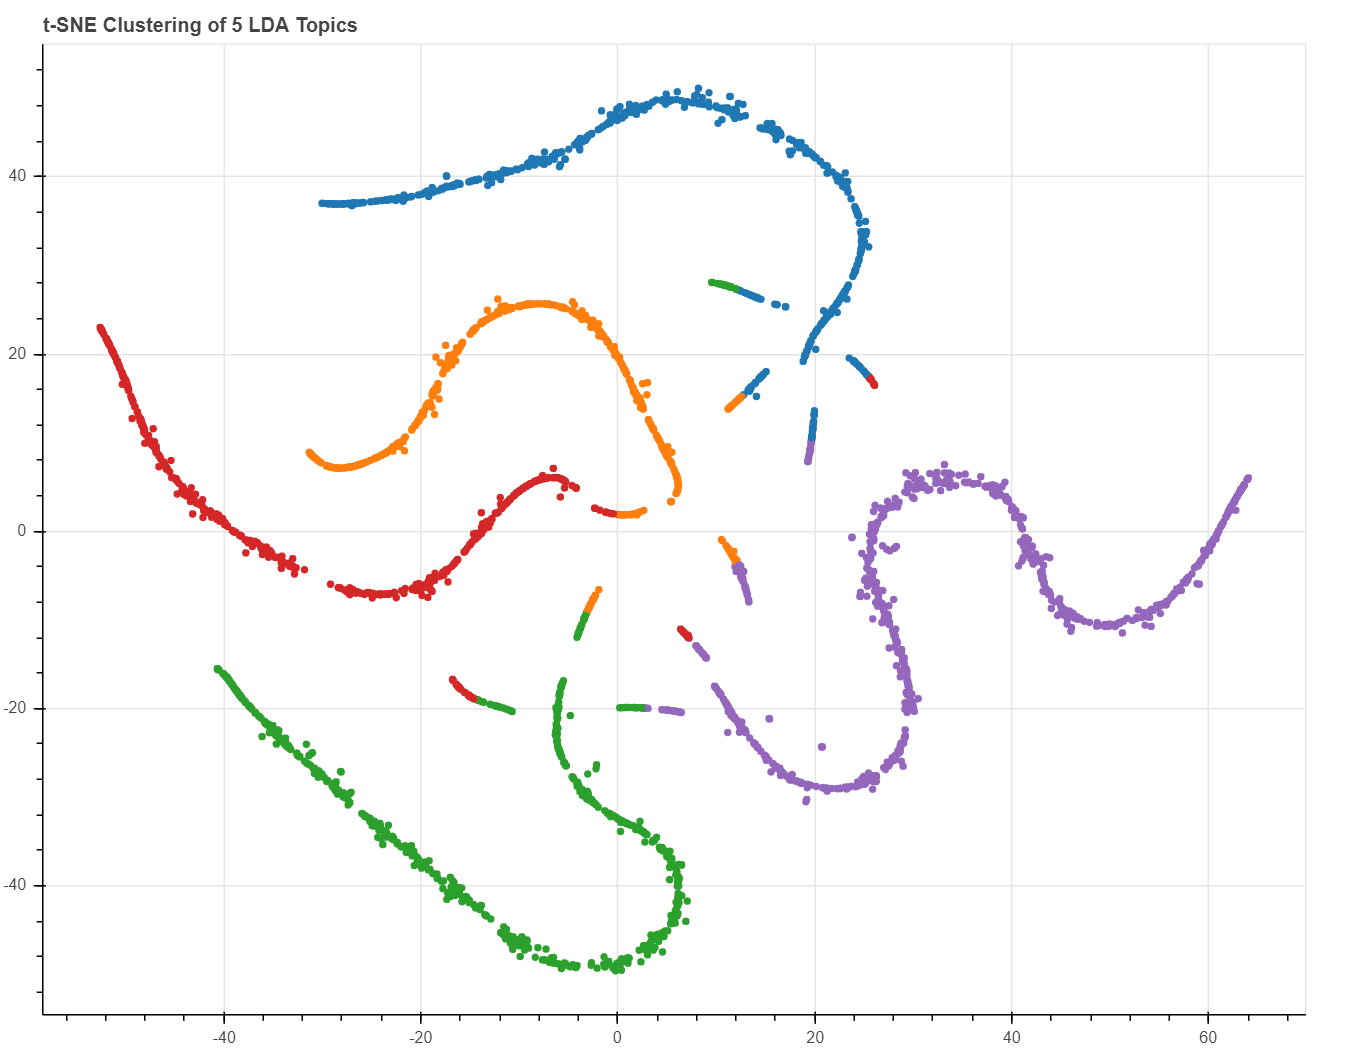
\includegraphics[width=0.49\textwidth]{screenshots/lda-tf-idf.png}}
    \subfigure[LDA Plot with colors for domains\label{fig:lda-tf-idf-domains}]{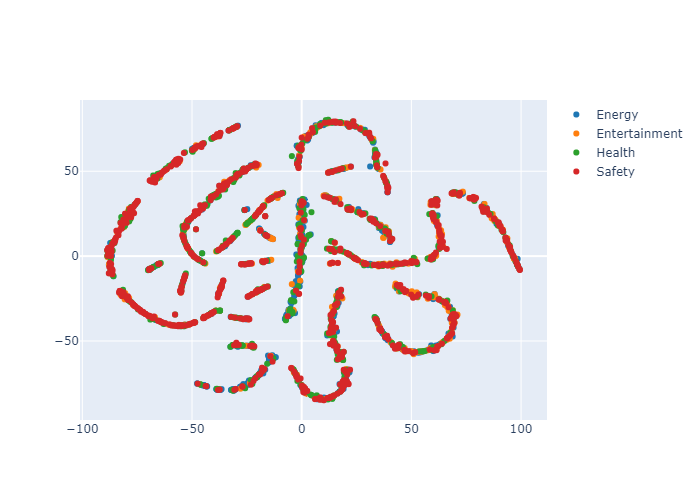
\includegraphics[width=0.49\textwidth]{screenshots/lda-domains.png}}
    \caption{LDA Result with TF-IDF (plotted with t-SNE)} \label{fig:lda-tf-idf}
\end{figure}
\FloatBarrier

In \autoref{fig:lda-tf-idf} we can see the result of the LDA that is plotted using t-SNE. In \autoref{fig:lda-tf-idf-topics} the colors are mapped to the found topics which of course looks better. But if we look for the expected mapping to the domains in \autoref{fig:lda-tf-idf-domains} we can see that the found cluster doesn't match to the expected ones.

\subsection{word2vec} % (fold)
\label{sub:own_word2vec}
For our word2vec approach, we made use of the gensim library\footref{fn:gensim_website}, which we mentioned in \autoref{sec:related_work} already and which was also used by Solangi et. al in \cite{solangi_review_2018}. We mainly used the \emph{gensim.models.Word2Vec} class, which implements both the CBOW and the skip-gram architecture of word2vec. We then followed different approaches, for the creation of our desired word embeddings. First, we tried to train our own model from the requiremnent senteces given the \crowdre{} dataset both with and without prior processing of the requirements through our NLP pipeline and on both architectures.\\
Being unsatisfied with the outcome, in a second attempt we created our embeddings using a pre-trained word2vec model, which contained the word vectors of a model trained on about 100 billion words of the Google News dataset\footnote{\url{https://code.google.com/archive/p/word2vec/}, last visited 2020-01-19}. Even though the outcome was different, the underlying workflow for both approaches was very similiar once the trained model was available:
\begin{itemize}
	\item For every tokenized requirement sentence, create a sentence matrix by replacing every word by its vector representation:\\
	$reqtokens = \{"As", "smart", "home", "owner", \dots\}$\\
	$embeddings = \{ \vec{as}, \vec{smart}, \vec{home}, \vec{owner}, \dots \}$
	\item On the resulting matrices, reduce the different x-dimensions to the dimension of the shortest sentence using Principal Component Analysis
	\item Use K-Means to generate a number of clusters on these now equally shaped matrices
	\item Visualize the results by transforming the data into 2d space using t-SNE\cite{maaten_visualizing_2008}
\end{itemize}


\begin{figure}[h]
  \begin{center}
    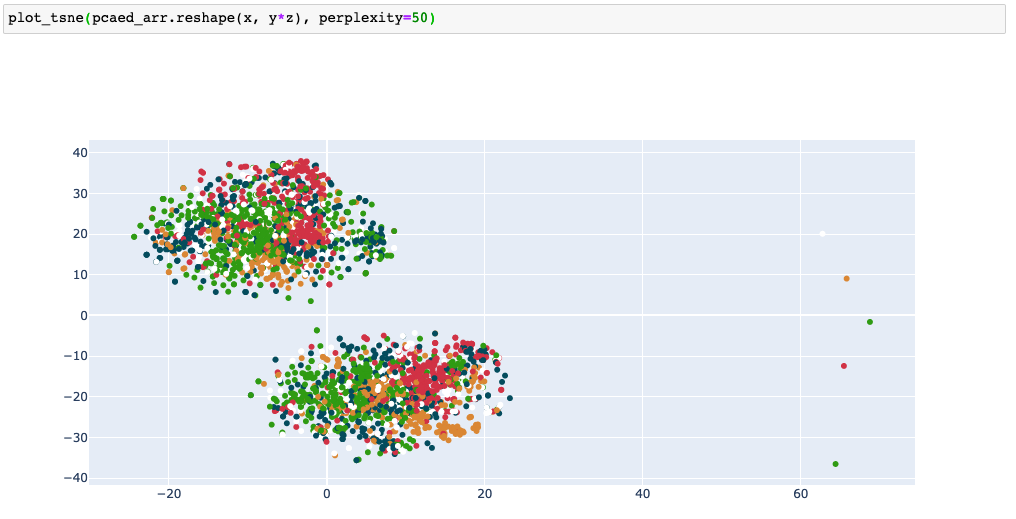
\includegraphics[width=\textwidth]{screenshots/google_word_2_vec_tsne_opti4.png}
    \caption{word2vec result of the clustering with a pretrained model (plotted with t-SNE)}
    \label{fig:w2v-pretrained-4}
  \end{center}
\end{figure}

\subsection{Word Mover's Distance} % (fold)
\label{sub:own_wmd}
Finally, we used the Word Mover's Distance which was also implemented in the gensim library. To do so, it was also necessary to create word embeddings for our requirement sentences first. Again, we could use the word vectors of the aforementioned word2vec models. Instead of basing our clusters on the distance between word vectors though, we could now calculate a distance matrix which holds the calculated Word Mover's Distance from every sentence to every other sentence, as represented in \autoref{tbl-wmd-matrix}. Note how the Word Mover's Distance is symmetric. So the distance to travel from $s_1$ to $s_2$ is the same as if your travelling vice versa.

\begin{table}[h]
\centering
\begin{tabular}{lllll}
             & $s_1$                      & $s_2$                      & $s_3$                      & ...                      \\ \cline{2-5} 
\multicolumn{1}{l|}{$s_1$} & \multicolumn{1}{l|}{0}    & \multicolumn{1}{l|}{0.83} & \multicolumn{1}{l|}{3.23} & \multicolumn{1}{l|}{...} \\ \cline{2-5} 
\multicolumn{1}{l|}{$s_2$} & \multicolumn{1}{l|}{0.83} & \multicolumn{1}{l|}{0}    & \multicolumn{1}{l|}{2.77} & \multicolumn{1}{l|}{...} \\ \cline{2-5} 
\multicolumn{1}{l|}{$s_3$} & \multicolumn{1}{l|}{3.23} & \multicolumn{1}{l|}{2.77} & \multicolumn{1}{l|}{0}    & \multicolumn{1}{l|}{...} \\ \cline{2-5} 
\multicolumn{1}{l|}{...}  & \multicolumn{1}{l|}{...}  & \multicolumn{1}{l|}{....} & \multicolumn{1}{l|}{...}  & \multicolumn{1}{l|}{0}   \\ \cline{2-5} 
\end{tabular}
\caption{Sentence Matrix containing the Word Mover's Distance from one sentence to another}\label{tbl-wmd-matrix}
\end{table}

 Since by its nature, the resulting matrix already was a 2-dimensional array with equal dimensions, it was not necessary anymore to perform any further reduction. We could use this matrix instead to directly create some clusters using K-Means.

 \begin{figure}[ht]
  \begin{center}
    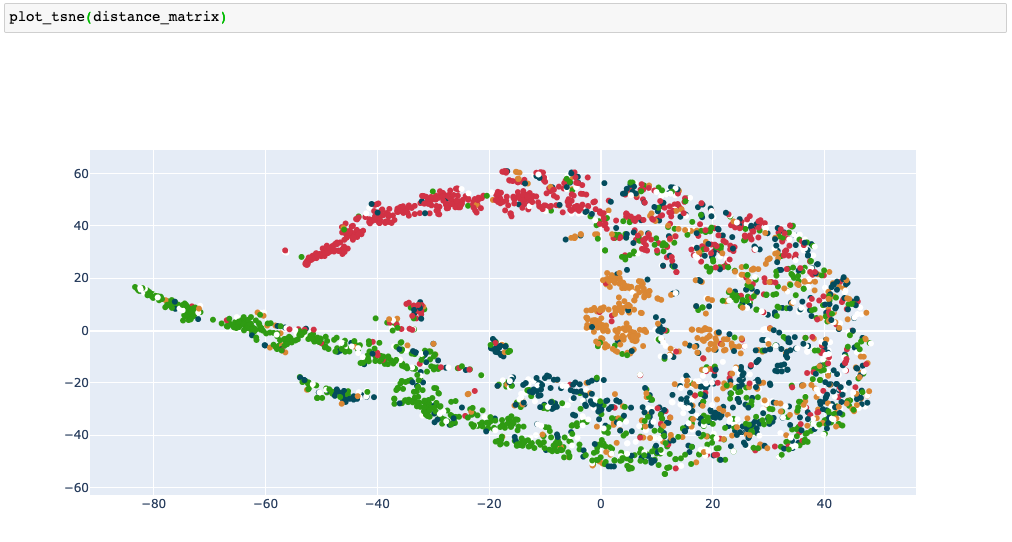
\includegraphics[width=\textwidth]{screenshots/our_word_movers_distance_tsne.png}
    \caption{Distance Matrix of the Word Mover's Distance with a self-trained model (plotted with t-SNE)}
    \label{fig:wmd-selftrained-1}
  \end{center}
\end{figure}